\documentclass{report}
\usepackage{graphicx}
\usepackage{amsmath}
\usepackage{epstopdf}
\usepackage[margin=1in]{geometry}
\usepackage{setspace}
\usepackage{amsthm}
\spacing{2}
\theoremstyle{definition}
\newtheorem{definition}{Definition}
\usepackage{epsfig}
\providecommand{\e}[1]{\ensuremath{\times 10^{#1}}}
\usepackage{float}

\usepackage{subcaption}



\begin{document}



\title{Solving the Schr\"odinger Equation Using Graphical Processing Units}
\date{\today}
\author{Johnny Minor \\Washington State University\\ Department of Physics and Astronomy %, Pullman Washington 99164}
}


\maketitle
%
%\begin{abstract}
%
%
%%gives a very brief indication of:
%%the aim of the report, 
%%what you did, 
%%what you found, 
%%what you concluded. 
%
%During the summer of 2014 with the guidance and supervision of Jared L. Aurentz and Mark G. Kuzyk I investigated different methods for computing the second order non-linear susceptibility. I first began programming the problem using Python. I then moved onto programming in MATLAB and finally in C and CUDA. We found that using the GPU(graphical processing unit) was faster at computing the solutions to the Schrödinger equation by a factor of 100 and is also more accurate by using Chebyshev Spectral differentiation. This new method for solving the Schrödinger equation seems to be a promising step towards faster and more accurate computational methods for, but not limited to, non-linear optic materials, and the quest for a beta greater than the fundamental limit. \cite{kuzyk2000physical}
%
%\end{abstract}


\section*{Introduction}
%provides the context for the report
%states why the topic is important or useful
%explains any abbreviations or special terms.

%From Tokyo to Los Angeles, from Pullman to Moscow fiber optic networks constantly connect people near and far into a massive instantaneous interconnected mesh. This modern feat of bringing people from massive distances away to your fingertips would not be possible without advancements in optics throughout the latter half of the 20$^{th}$ century. As the sun sinks below the horizon in Tokyo it is just beginning to rise in Los Angeles. As old technologies fade away the  research fin nonlinear optics brightens. 


During the summer of 2014 with the guidance and supervision of Jared L. Aurentz and Mark G. Kuzyk I investigated different methods for computing the second order non-linear susceptibility. I first began programming the problem using Python. I then moved onto programming in MATLAB and finally in C and CUDA. We found that using the GPU(graphical processing unit) was faster at computing the solutions to the Schrödinger equation by a factor of 100. This is a good speed up for computational time. A further benefit of computing on the GPU is that they are readily accessible to the general public in comparison to a computer cluster which may be similar in computational time for these types of problems. Also, this would allow for researchers to quickly find solutions to their problems rather than relying on computational models which can frequently take hours or days to finish. 

This new way of solving the Schr\"odinger equation is further accentuated by a more accurate way of calculating $\beta$, the hyperpolarizability -- a quality of importance to elctro optical switch. We have used the Chebyshev Spectral differentiation method on the polarization function, a spectral method that offers much greater accuracy and precision in computations. This is an important aspect of the calculation of $\beta$ for polarization functions which may not be so smooth, and therefore making them more difficult to approximate for a finite difference method. This is also important becausej increases confidence in the precision of the results. 

This new method for solving the Schr\"odinger equation seems to be a promising step towards faster, and more accurate computational methods for, but not limited to, non-linear optic materials, and the quest for a $\beta$ that approaches the fundamental limit. \cite{kuzyk2000physical}


\subsection*{History}

A nonlinear optical response is induced by a laser beam in a medium as a function of the applied electric and magnetic fields. \cite{bloembergen}. Generally, lasers are used as they have high enough intensity to induce the displacement of charges in proportion to a nonlinear function of the electric field. For instance second-harmonic generation scales quadratically in relation to the applied optical field lead to frequency double, where for example red light is converted to green light--a common way to make green laser pointer from less expensive red laser diodes. Stated alternatively, nonlinear optics is the interaction of a laser with a material, and the understanding of how the phenomena that result.

Nonlinear optics was born in the early 1960's when Franken \textit{et al.} passed a ruby laser through a quartz crystal and noticed that the emitted ultraviolet radiation was in fact twice the frequency than that which entered the crystal. Building upon this rather startling discovery Maker \textit{et al.} and Giordmaine in 1962 improved, by many orders of magnitude,  the second harmonic generation efficiency by matching the phase of the fundamental and harmonic wae using compensation of the color dispersion by birefringence in an anisotropic KDP crystal. \cite{bloembergen} From those early years in the 1960's the field of nonlinear optics has grown immensely into a mature and rich field with a broad range of applications ranging from quantum optics, nonlinear spectroscopy, and nonlinear optical materials.% to the area of which Professor Mark Kuzyk and his collaborators investigate-nonlinear optic materials. 

%Now, nonlinear optics can be understood 

%\begin{figure}
%\begin{center}
%\includegraphics[width=.5\textwidth]{lasers.jpg}
%\caption{Researchers observe nonlinear optic phenomena}
%\end{center}
%\end{figure}


\subsection*{Quantum Mechanical Origins of Nonlinear Optics}

Nonlinear optic phenomena can be understood macroscopically using Maxwell's Equations that describe electromagnetic theory. However, quantum mechanics offers an understanding of the origins of the nonlinear, and makes numerical predictions of the nonlinear susceptibilities. \cite{boyd2003} The basis of quantum mechanics is the Schr\"odinger equation. It can take a myriad of forms depending on the conditions of the problem being solved. The specific form which is of most interest to us is the time-independent Schr\"odinger equation in one dimension,

\begin{equation}
\lambda \psi(x) = \left[ \frac{-\hbar^2}{2m}\frac{\partial^2}{\partial x^2} + V(x) \right] \psi(x)
\end{equation}

\noindent where $\lambda$ is the energy eigenvalue, $\psi(x)$ is the wave function(eigenfunction), $\hbar\ = h/2\mathrm{m}$ is reduced Planck's constant, m is the mass of an electron, $V(x)$ is the potential operator. %, and $E(x)$ is the electric dipole moment operator.

However, this equation of continuous variables must be discretized to make it solvable on a computer.Therefore, the discrete grid mesh must be defined, for the finite set of x-values which the function spans. This grid mesh is frequently defined by a right endpoint, a left endpoint, and a number of points within that domain. The equispaced grid mesh is 

\begin{equation}
\mathrm{interval \; length = (right \; endpoint - left \; endpoint) / number \; of \;  points \; + \; 1}.
\end{equation}

 \noindent Once these points are defined, the linear operators can be created. Furthermore, once the problem has been discretized it becomes a matrix eigenvalue problem.\cite{watkins2004fundamentals} The Schr\"odinger equation then takes the form  % The electric dipole moment operator is varied using corresponding Chebyshev points and therefore you get a new Hamiltonian every time. reducing to 

\begin{equation}
\lambda \, \psi(x) = H \psi(x) 
\end{equation}  

\noindent where $\lambda$ is the eigenvalue and $\psi$ is the corresponding eigenvector of the defined Hamiltonian. 

\noindent The scheme for computing the polarization is to compute the wave function $\psi(x)$ as a function of the electric field E using the dipole potential $V(x) = -exE $ where $-ex$ is the dipole operator. For each field E, the Hamiltonian operator has unqiue eigenvectors. The ground state eigenvector is used to determine the induced dipole moment by determinging the ground state expectation value given by:

\begin{equation}
P(E) = \left\langle\mathrm{X} \psi(E) | \psi(E) \right\rangle ,
\end{equation}

where $\psi$ is the ground state eigenvector of the Hamiltonian and $X$ is the position operator(specified on the domain). This yields the induced dipole moment as a function of the applied electric field. The second derivative gives $\beta$ according to:

\begin{equation}
\beta = \frac{1}{2}\frac{\partial p^2}{\partial E^2}\bigr|_E=0
\end{equation}




\subsection*{Recent Research}

Professor Mark G. Kuzyk and his many collaborators have been investigating the limits of the second order non-linear susceptibility for over a decade. He originally published a paper in 2000 which derives the fundamental limit for beta which takes the form \cite{zhou2007}

\begin{equation}
\beta_{\max} = \sqrt[4]{3} {\left( \frac{e\hbar}{\sqrt{m}} \right)\!\!}^3 \frac{N^{3/2}}{E_{10}^{7/2}}    
\end{equation}

\noindent where N is the number of electrons, $E_{10}$ is the energy of the first excited state, m is the mass of an electron, and $\hbar$ is the reduced Planck's constant. A scale invariant quantity can be used to compare molecules of different sizes is called the intrinsic hyperpolarizability given by, 

\begin{equation}
\beta_{int} = \frac{\beta}{\beta_{max}},
\end{equation}

\noindent Where $\beta$ is the computed value and $\beta_{max}$ is the limit of the hyperpolarizability \cite{kuzyk2000physical}. Since 2000 researchers around the world have been attempting to find a $\beta_{int}$ greater than one, and they have all fallen short of the fundamental limit. % that Professor Kuzyk has presented. %Quite interestingly the $\beta$ which we found to be the highest is the identitcal to those found in 2007 by Zhou et al. of 0.704 or $\frac{1}{\sqrt{2}}$


\subsection*{Research Goals}

The primary tool for attempting to discover a $\beta_{int}$ greater than one is through computational methods. Computational Physics is a fast paced and promising realm for the future, and algorithms for solving such a Physics problem are at the forefront of the modern-era.  What Jared Aurentz and I set out to do was to create an algorithm that had parameters which could be changed relatively easily, and that would correspond to a new Hamiltonian. With this newly defined Hamiltonian it would be possible to compute $\beta$ quickly. This would help Professor Kuzyk's team of researchers by being able to computationally simulate many different systems without having to experimentally create them. We had hoped, if possible, to find a system which would give characteristics that would give a $\beta_{int}$ value approaching unit if not larger than one. This would give chemists and experimentalists the direction for creating the physical properties analogous to the computational model. 


\section*{Method}
%sets out what you did in sequence ,
%explains how you did it
%indicates what materials, techniques or equipment you used
%provides sufficient information for the reader to replicate the study.

\subsection*{Computing In Python}
At the beginning of the summer I first began investigating the hyperpolarizability $\beta$ by numerically solving the Schr\"odinger equation in the high-level programming language Python. As I stated previously, the Schr\"odinger equation must be discretized in order for it to become solvable on a computer. This means that the Schr\"odinger equation becomes a synthesized matrix of the derivative operator and the potential operator over a specified domain. These operators are then added together element-wise and the scalars are multiplied in. The problem can then be solved using matrix eigenvalue methods.

In order to accomplish computing $\beta$ successfully I relied heavily on the additional linear algebra functions included in the  Sympy library. This allowed for much quicker and easier creation and manipulation of vectors and linear operators. In order to discretize the continuous time independent Schr\"odinger equation a finite-difference technique was used for discretizing the second derivative operator.

For example the discretized second derivative operator using a finite difference method for discretization takes the form\cite{watkins2004fundamentals}: 

\[-\frac{\partial^2}{\partial x^2} \qquad \mbox{becomes} \qquad \Delta = - \left( \begin{array}{c c c c}
2 & -1 & & 0\\
-1 & \ddots & \ddots & \\
& \ddots & \ddots & -1 \\
0 & & -1 & 2 \end{array} \right) \],

\noindent and the harmonic oscillator $x^2$ potential takes the form 

\[
V(x) \qquad becomes \qquad  \widehat{ V}= \left( \begin{array}{cccc}
   -0.6\\
    & -0.2 &  & \text{\huge0} \\
    & & 0.2\\
    & \text{\huge0} & & 0.6\\
 \end{array} \right) 
\],


Where for illustration we use the interval from [-1,1] with 4 points since the endpoints are zero, they are left out. 
A discrete equispaced domain was also created using Python. This was needed in order to define the operators that relied upon the x values. Once the resulting Hamiltonian operator was created,  then the eigenvalues and eigenvectors were computed using a familiar power iterative method for solving the matrix eigenvalue problem. The eigenvalues and eigenvectors are then used to compute $\beta$ by using sum-over-states($\beta_{SOS}$)\cite{kuzyk2005compact, orr1971perturbation}.The sum-over-states expression requires that enough eigenvalues and eigenvectors are used for the sum to converge usually, about 15 states are sufficient for $\beta$ to converge, which can be tested by comparing numerical with analytical results \cite{kuzyk2005compact}.This is an important difference between the derivative method $\beta_{SOS}$)  This of course gave the familiar value of $\beta_int$ = 0.57 for the  clipped quantum harmonic oscillator potential($x^2$). %could add more details about what SOS is and how to compute it etc. 

\subsection*{Computing In MATLAB}
After I had a feel for computing $\beta$ we moved to computing it using MATLAB. Thanks to the hard work of Nick Trefethen and his team of developers at the University of Oxford the use of the Chebfun package was incalculably beneficial \cite{chebfun}.

One of the most prominent differences between Chebfun and other methods of finite differences, is that it instead uses spectral interpolation. This requires much fewer points, and as we will see, is much more accurate than a finite difference method\cite{trefethen2000spectral}. 

Using Chebfun gives an intuitive and simple way of programming differential equations, such as the Schr\"odinger equation, in MATLAB. A quick example of the power and simplicity of Chebfun is that it's possible to compute the solutions to a simplified Schr\"odinger equation with only four lines of MATLAB code as follows: 


\bigskip
% here is some computer code

\begin{minipage}{5in}
\noindent
%{\Large Solving The Schr\"odinger Equation Using Chebfun}
\begin{verbatim}
L = 10;
dom = [-L,L];
d2 = chebop(@(x,u) -diff(u,2) + x.^2.*u, dom, 'dirichlet');
[V,D] = eigs(d2,1,0); plot(V(:,1)); norm(V(:,1),2);
\end{verbatim}
\end{minipage}

\bigskip


\noindent It is important to notice that Chebfun bypasses the need to create matrices explicitly. It has this process automated. It interpolates with increasing number of Chebyshev points until the accuracy converges to machine precision(1\e{-16}). This is incredibly handy because the interpolated matrices will not be sparse matrices like the $\Delta$ and $\hat{V}$ matrices in Python. This incredible feature can be leveraged rather nicely to compute $\beta$ efficiently. However, using polynomial interpolation through Chebyshev points(hence the name 'Chebfun'), and the associated grid mesh we were able to retain twice as much fidelity in our computation in comparison with that of using Python. When using the finite difference method we would only be able compute solutions to the Schrodinger equation with about six significant figures whereas using spectral methods we were able to compute eigenvectors to machine precision. Since we were able to compute the eigenvalues and eigenvectors so precisely we were also able to carry this precision further in the computation. This was very beneficial because data is lost when a derivative is taken which is compounded when taking the second derivative. This meant that we would be more accurate in our calculation of $\beta$. In order to match this precision using a finite difference method would not be practical because the domain would have to be increased to an astronomically small grid mesh that would correspond to a massive number of points, and a problem of such a magnitude is seemingly not computational feasible. 

For comparison we created a similar algorithm to optimize $\beta_{int}$ using a similar method to that which Zhou, Kuzyk and Watkins implemented in 2007.\cite{zhou2007} Instead this time we used spectral methods instead of quadratic finite element and optimized using the same Nelder-Mead simplex optimization function call in MATLAB. This test yielded similar results to those found by Zhou, Kuzyk, and Watkins. However, the solutions are more precise by about 2 significant figures. 

\subsection*{Computing In C}
Finally, we programmed the discrete time independent Schr\"odinger equation using C,  a low-level language that offers many hurdles for a beginner programmer. We were able to overcome these challenges. Not only was the manipulation of data a challenge but also many(nearly all) of the packages I had grown to know and love in the higher-level languages such as Python and MATLAB had to be written by myself. They had to be engineered in such a way to take an arbitrary size array. This meant learning about dynamic memory allocation. Furthermore, I had to create numerous functions such as: trapezoidal integration, inner product, normalization of an array, creating the laplacian operator, the potential operator, and the electric field operator. One by one the functions were created, tested (de-bugged), and implemented into the final program. 

Where things became even more interesting was through the differentiation of the polarization function. Since we used a spectral method interpolation for approxmating the function we had to use spectral method differentiation matrix for computing $\beta$ instead of using a more traditional route\cite{trefethen2000spectral}. With the spectral method differentation matrix code created we were able to take the second derivative of the polarization function, which would in turn give us $\beta$ for the associated Hamiltonian. 



\subsection*{Implimentation Of Spectral Methods}

 Spectral methods are rooted in Chebyshev interpolation. Where a function is approximated using specific points and interpolating through them with a polynomial.With spectral methods, instead of using an equispaced grid of points you must generate the points on the domain. Picking the grid points in such a manner is what truly makes spectral methods special. This method has been developed extensively from \cite{trefethen2000spectral,trefethen2013approximation} as well as from \cite{welfert1997generation}. 
 
 The Chebyshev grid points can be defined as follows on an interval from [-1,1]:


\begin{definition}[Chebyshev points of the first kind]

\begin{equation}
x_{j} = \cos(j \pi / n), \qquad  0 \leq j \leq n, 
\end{equation}

\end{definition}


\noindent where n is the number of chebyshev points and j is the index value. The optimal number of Chebyshev points, which is outside of the scope of this humble report and won't be discussed, is specified to be $2^{n}+1$. For instance, the number of chebyshev points you would want would be $2^{1}+1$ or $2^{2}+1$ and so on. Hence why I will use three and five Chebpoints below. This is also important considering we would need an odd number of points in order to confidently compute the derivative at zero on the domain we're interest in. An arbitrary function $f(x) = -\sin(7x)^{\cos(3x-1)}+5x+1$ is used for illustrative purposes to highlight just how quickly the Chebyshev interpolation converges to an arbitrary function. 


\begin{figure}[H]
\centering
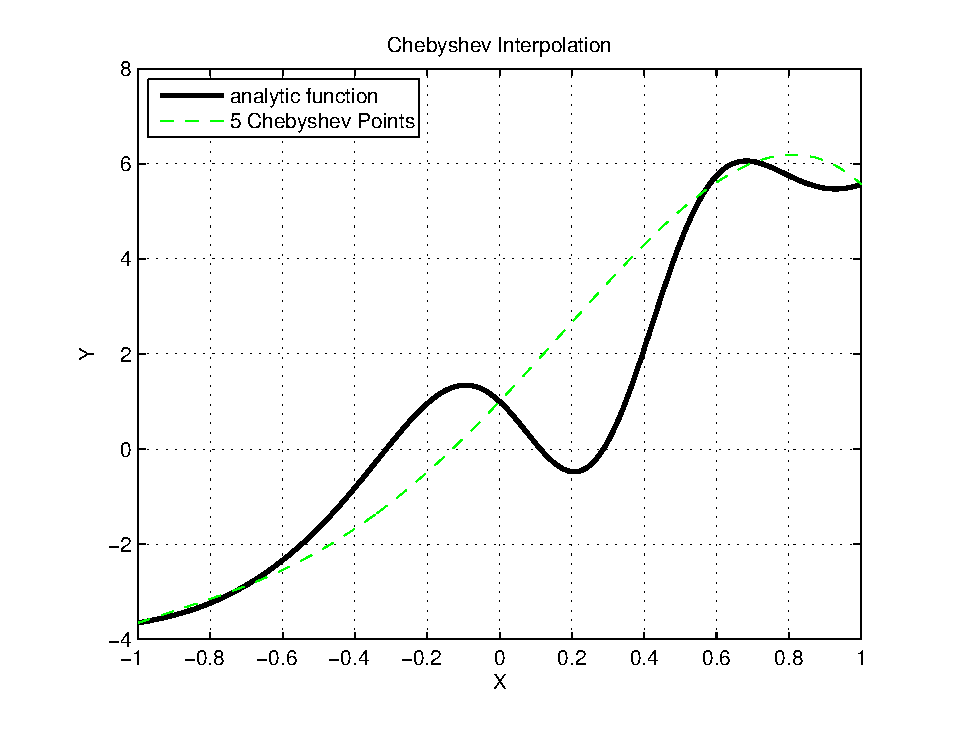
\includegraphics[width=.6\textwidth]{5chebpts.eps}
\caption{Interpolant using Five Chebyshev Points.}
\label{fig:digraph}
\end{figure}

\begin{figure}[H]
\centering
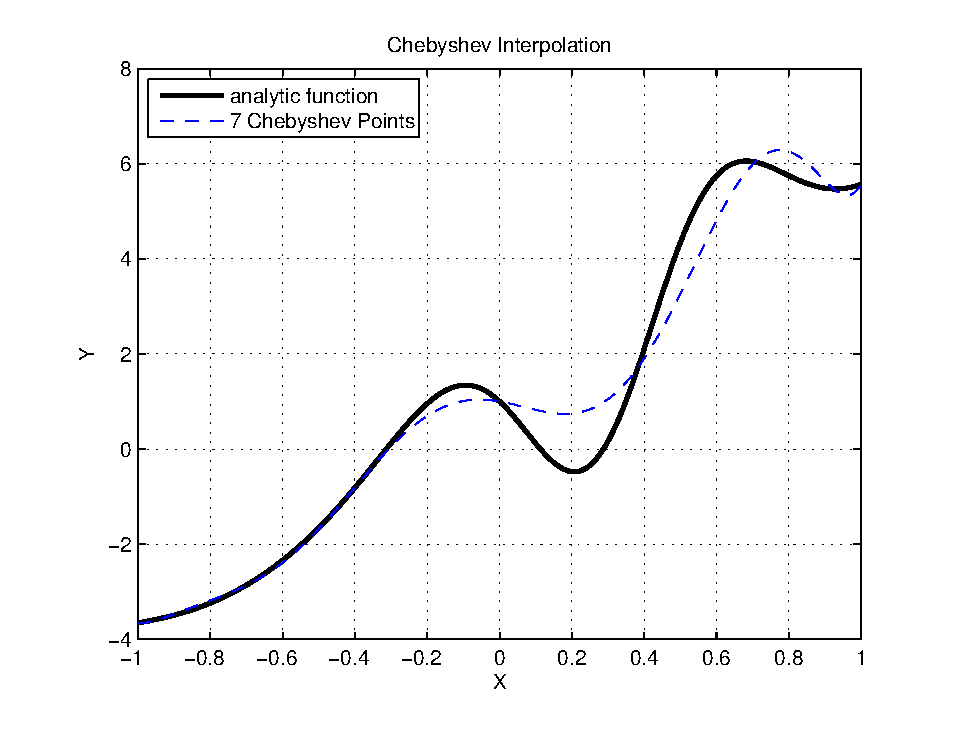
\includegraphics[width=.6\textwidth]{7chebpts.eps}
\caption{Interpolant using Seven Chebyshev Points. }
\label{fig:digraph}
\end{figure}

%\end{array}

\begin{figure}[H]
\centering
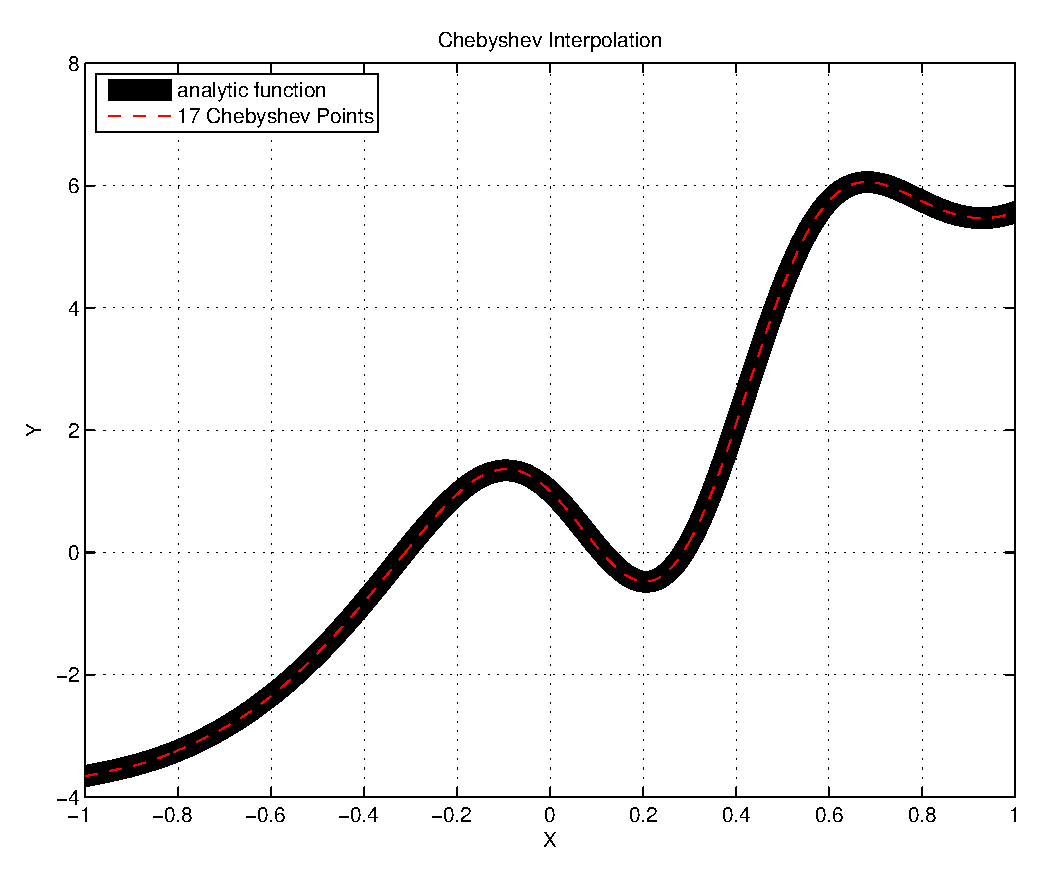
\includegraphics[width=.5\textwidth]{17chebpts.eps}
\caption{Interpolant using 17 Chebyshev Points. }
\label{fig:digraph}
\end{figure}





%
%\begin{figure}
%\centering
%\begin{subfigure}{.8\textwidth}
%  \centering
%  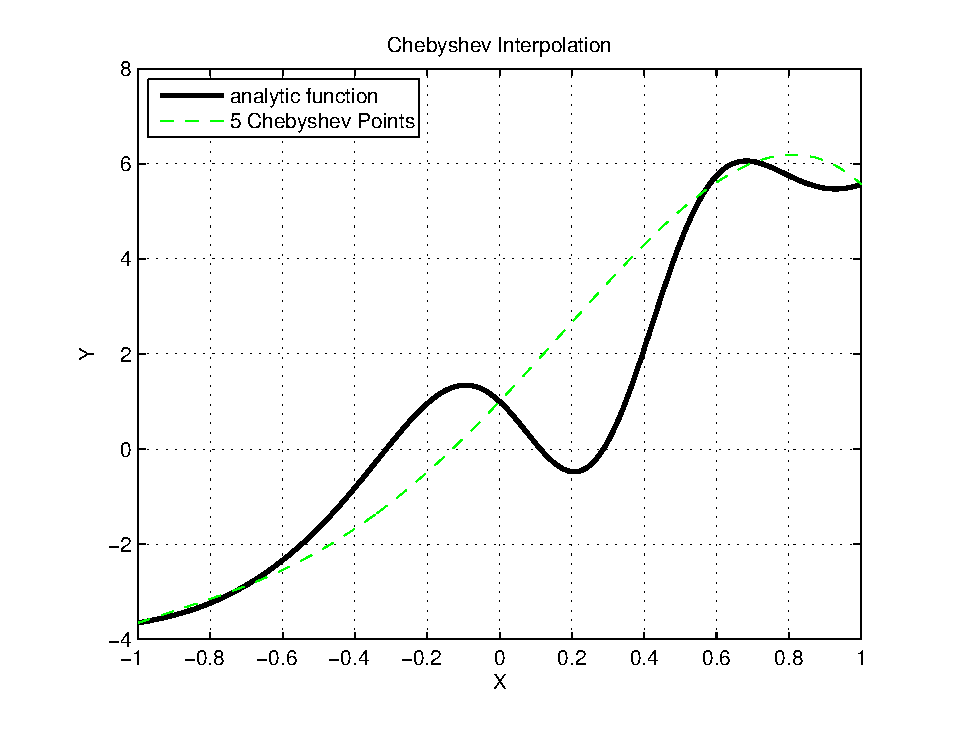
\includegraphics[width=.2\linewidth]{5chebpts.eps}
%  %\caption{A subfigure}
%  \label{fig:sub1}
%\end{subfigure}%
%\begin{subfigure}{.8\textwidth}
%  \centering
%  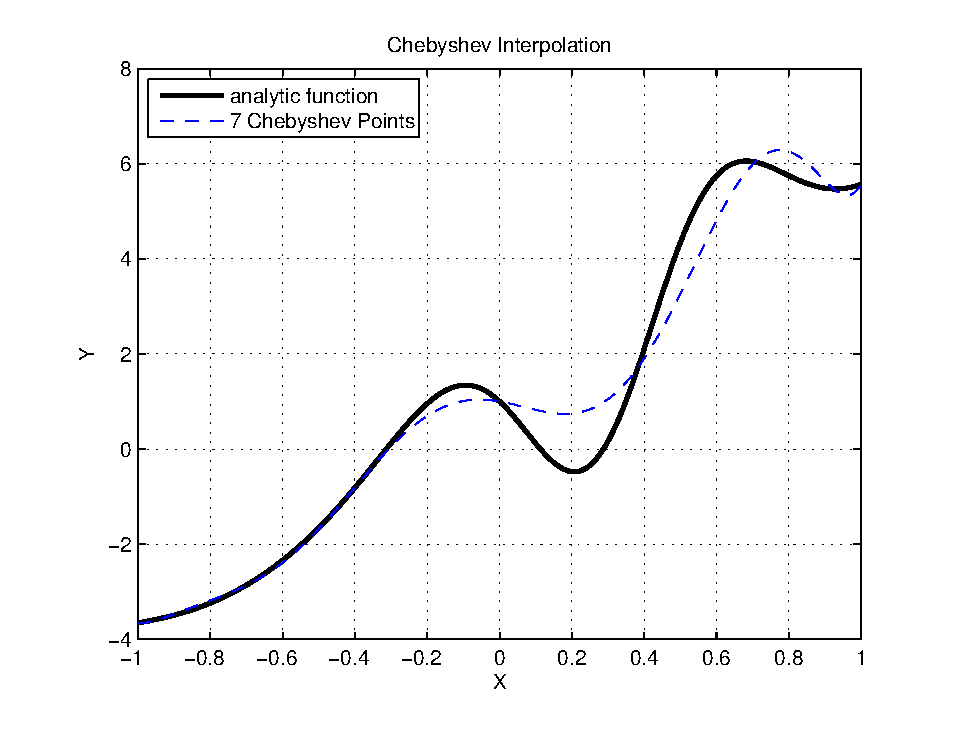
\includegraphics[width=.2\linewidth]{7chebpts.eps}
%  %\caption{A subfigure}
%  \label{fig:sub2}
%\end{subfigure}
%%\caption{A figure with two subfigures}
%\label{fig:test}
%\end{figure}

By using a mere 17 Chebyshev points we can already hardly tell a difference visually between the analytic function and our Chebyshev polynomial interpolant. Using Chebfun we can see that after a mere 55 Chebyshev points the polynomial interpolant is at machine precision(1\e{-16}).

 With these Chebyshev points we can interpolate our computed polarization values using Lagrangian interpolation. The Lagrange form is a linear combination of Lagrange polynomials: 

\begin{equation}
p(x) = \sum_{j=0}^{n} f_{j}\ell_{j}(x),
\end{equation}

\noindent where x is the set of interpolation points(chebyshev points) and $l_{j}$ is the $j$th Langrange polynomial that's unique and has the value of 1 at $x_{j}$ and is 0 at all points $x_{k}$

\begin{equation}
\ell_{j}(x_{k}) = \left\{ 
  \begin{array}{l l}
    1, & \quad k = j \\
    0, & \quad k \neq j \\
  \end{array} \right.
\end{equation}

%this can be illustrated by an image. 
%
%\begin{figure}[H]
%\centering
%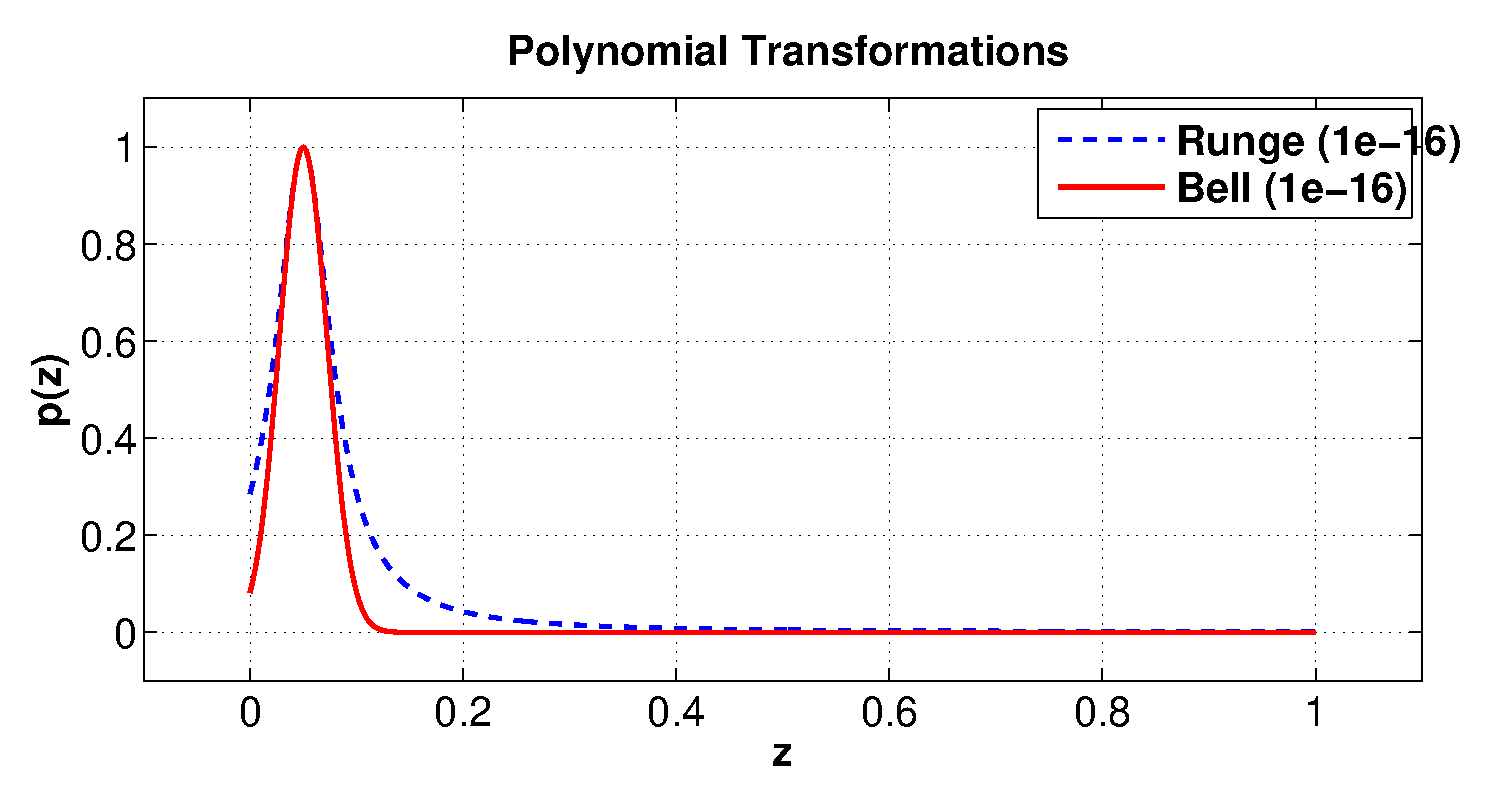
\includegraphics[width=.9\textwidth]{Figures.eps}
%\caption{$\sqrt{J}$ graph }
%\label{fig:digraph}
%\end{figure}


%% here is some computer code
%
%\begin{minipage}{5in}
%\noindent
%{\Large Solving The Schr\"odinger Equation Using Chebfun}
%\begin{verbatim}
%L = 10;
%dom = [-L,L];
%d2 = chebop(@(x,u) -diff(u,2) + x.^2.*u, dom, 'dirichlet');
%[V,D] = eigs(d2,1,0); plot(V(:,1)); norm(V(:,1),2);
%\end{verbatim}
%\end{minipage}
%
%\bigskip

This is a key element in the differentiation of computing the second derivative of the polarization function. Since we have interpolated our polarization function with Lagrangian polynomials we then can take the second derivative at x = 0 in order to find $\beta$. We use a Chebyshev differentiation matrix with entries 

\begin{equation}
\begin{array}{c c}
(D_{N})_{00} = \frac{2N^{2}+1}{6} & \qquad \qquad (D_{N})_{NN} = \frac{2N^{2}+1}{6} \\
\end{array}
\end{equation}


\begin{equation}
(D_{N})_{jj} = \frac{-x_{j}}{2(1-x_{j}^{2}} \qquad \qquad j = 1,\dots,N-1
\end{equation}

\begin{equation}
(D_{N})_{ij} = \frac{c_{i}}{c_{j}} \frac{(-1)^{i+j}}{(x_{i} - x_{j})}, \qquad \qquad i \neq j, \quad i,j = 0,\dots, N,
\end{equation}

\textit{where}

\begin{equation}
c_{i} = \left\{ 
  \begin{array}{l l}
    2, & \quad i = 0\; or \; N \\
    1, & \quad otherwise.\\
  \end{array} \right.
\end{equation}

By constructing this matrix and multiplying it by itself element-wise we get the second derivative spectral matrix. Taking the product of it with the vector full of polarization values we are able to compute $\beta$. 



\subsection*{Computing With A GPU}
Graphical Processing Units were primarily used for video games. They were intended to manipulate the vector rendered graphics quickly and efficiently. This fact can be leveraged for scientific computing. In order to do this with NVIDIA GPU's requires a low level language named CUDA. CUDA is syntactically quite similar to modern C++ standard. However, memory management plays a key role, and  programming in CUDA  requires the programmer be cognizant of whether the data is on the CPU or on the GPU. Without careful attention the already tricky programming can become an arduous process of debugging. CUDA has a handful of elementary functions built-in for manipulating linear algebra type data. %However, a much quicker algorithm for solving the eigenvalues and eigenvectors would be essential to the computation of $\beta$. 

One aspect of computational physics is that increased accuracy and precision requires an increase in the amount of data which is being processed. In a linear system this can often approach the millions of unknowns using a finite difference approximation scheme. However, the computational time for such a calculation can often take hours, and perhaps even days depending on the calculation or simulation being run. 

%Furthermore, as I found first hand this summer, that finite difference approximation is truly a poor approximation and only becomes worse as the data gets manipulated further.  

This is where computations on the GPU truly shine. The GPU can take problems that seem incomputable and making implementation possible and taking only a few minutes. This is greatly advantageous because researchers can get results quickly. 

Previously we had used LAPACK's eigen-solver to compute the solutions to the discretized Schr\"odinger equation, but with the introduction of Jared's recently completed eigen-solver we were able to implement his packages and begin off-loading much of the computations to the GPU. This reduced computational times dramatically. 






%\section*{Numerical Examples}
%presents what you found
%includes clearly titled and labelled graphs, tables and figures as appropriate
%do not simply cut and paste an Excel file into your document
%detailed calculations may be provided in the appendix.
We found implementing Jared's eigen-solver dramatically reduced the time. We can now compute much larger problems that we previously thought would be nearly impossible. 




%\section*{Discussion}
%explains what the results mean
%indicates whether the results were consistent or inconsistent with your expectations
%explains what possible sources of error there are
%indicates how the experiment could be improved in future.
The results mean that we can compute the eigenstates of the quantum harmonic oscillator very fast and with relatively good accuracy. This seems very promising for larger problems with hundreds of thousands of points. the error could be brought down significantly if the spectral interpolation was written for C instead of using finite difference. 





\section*{Conclusion}
%briefly restates the main results
%briefly explains the significance of the findings.
We found implementing Jared's eigen-solver dramatically reduced the time. We can now compute much larger problems that we previously thought would be nearly impossible. 


The results mean that we can compute the eigenstates of the quantum harmonic oscillator very fast and with relatively good accuracy. This seems very promising for larger problems with hundreds of thousands of points. the error could be brought down significantly if the spectral interpolation was written for C instead of using finite difference. 



Optimistically the goal was set to create an algorithm to test many different Hamiltonians and check the corresponding $\beta$. Currently we are still working on implementation on the GPU in computing $\beta$, and we are nearing a first milestone of finally implementing the C code which I wrote with Jared's eigensolver, but at this time I unfortunately don't have any concrete numerical examples. Although this goal was not reached a prodigious amount of progress was made not only regarding this project, but also for my own understanding of Professor Kuzyk and his collaborators work as and their contributions to the field of nonlinear optics. 

All of these problems have been elementary, but the focus of the research this summer was to develop new ways of solving the Schr\"odinger equation. As we have found the new method of parallelization of solving the Schr\"odinger equation yields an impressive advantage of speed. Although this is only one instance it could be a promising alternative if it could be implemented in a higher level language and therefore making it more accessible to researchers. Furthermore, the range of applications is massive considering differential equations are used from engineering to the social sciences and throughout. With the amount of data increasing rapidly in today's world it is ever-more important to find solutions for dealing with this stupendous amount of data. 




%\section*{References}
%provides a list of sources of information which you have used, following the referencing conventions required for the unit (see Referencing).



%\section*{Appendices}

%provides supporting information such as calculations.



\bibliographystyle{plain}
\bibliography{NLO}


\end{document}